% SC2000 — Chapter 7: Estimation & Confidence Intervals
\chapter{Estimation \& Confidence Intervals}
\label{ch:estimation}

\begin{quote}
\emph{``Data is not information until it is estimated with uncertainty.''} A single number (``average latency $42\,$ms'') is meaningless without ``$\pm3\,$ms with $95\%$ confidence.'' Estimation turns samples into guesses; confidence intervals quantify how much to trust them.
\end{quote}

\noindent\fbox{\parbox{\dimexpr\linewidth-2\fboxsep-2\fboxrule}{%
\textbf{From zero: samples $\to$ guesses $\to$ guarantees.} We assume i.i.d.\ samples from an unknown distribution. Point estimators guess the parameter; interval estimators add an error bar whose coverage probability we control. CLT (Ch.~6) powers the intervals.}}
\vspace{0.4em}

\section*{Learning Outcomes}
After this chapter you will be able to:
\begin{enumerate}[label=(L\arabic*)]
    \item define bias, variance, and MSE and compute them for common estimators;
    \item derive MLEs for Bernoulli, Poisson, and Normal models;
    \item construct $z$- and $t$-confidence intervals for means and proportions;
    \item interpret ``$95\%$ confidence'' correctly (and spot misinterpretations);
    \item choose sample size to achieve a target margin of error.
\end{enumerate}

% ============================================================
\section{Point Estimation: Bias, Variance, MSE}
\label{sec:point-estimation}
We observe i.i.d.\ $X_1,\dots,X_n\sim f(x;\theta)$ with unknown $\theta$. An \emph{estimator} $\hat\theta=\hat\theta(X_1,\dots,X_n)$ is a function of the data (hence random).

\begin{definition}[Bias, variance, MSE] Bias$(\hat\theta)=\mathbb{E}[\hat\theta]-\theta$. $\hat\theta$ is \emph{unbiased} if bias $=0$. Mean squared error
\[
\mathrm{MSE}(\hat\theta)=\mathbb{E}[(\hat\theta-\theta)^2]=\mathrm{Var}(\hat\theta)+\text{Bias}^2.
\]
\end{definition}

Example: sample mean $\bar X=\frac1n\sum X_i$ is unbiased for $\mu$ ($\mathbb{E}[\bar X]=\mu$, $\mathrm{Var}(\bar X)=\sigma^2/n$). Sample variance $S^2=\frac1{n-1}\sum(X_i-\bar X)^2$ is unbiased for $\sigma^2$ (Bessel's correction); the MLE variant with $1/n$ is biased low.

Trade-off: shrinking an unbiased estimator toward $0$ introduces bias but can reduce MSE (bias--variance trade-off, central to ML).

\begin{figure}[h]
\centering
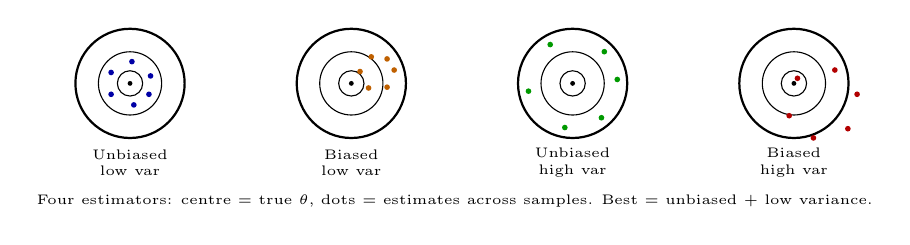
\begin{tikzpicture}[scale=0.73,every node/.style={font=\scriptsize}]
% Bias-variance targets
\foreach \idx/\labA/\labB/\col in {0/Unbiased/low var/blue,1/Biased/low var/orange,2/Unbiased/high var/green,3/Biased/high var/red} {
  \begin{scope}[xshift=\idx*3.85cm]
  \draw[thick] (0,0) circle (0.95);
  \draw[thin] (0,0) circle (0.55);
  \draw[thin] (0,0) circle (0.22);
  \fill[black] (0,0) circle (1.2pt); % true theta
  \node[font=\tiny,align=center] at (0,-1.38) {\labA\\ \labB};
  \ifnum\idx=0
    \foreach \a in {20,85,150,210,280,330} {\fill[blue!65!black] (\a:0.38) circle (1.4pt);}
  \fi
  \ifnum\idx=1
    \foreach \a in {10,55,110,175,240,305} {\fill[orange!75!black] (0.45,0.18) ++(\a:0.30) circle (1.4pt);}
  \fi
  \ifnum\idx=2
    \foreach \a in {5,45,120,190,260,310} {\fill[green!60!black] (\a:0.78) circle (1.4pt);}
  \fi
  \ifnum\idx=3
    \foreach \a in {15,70,135,200,255,315} {\fill[red!70!black] (0.50,-0.35) ++(\a:0.62) circle (1.4pt);}
  \fi
  \end{scope}
}
\node[font=\tiny,align=center] at (5.65,-2.05) {Four estimators: centre $=$ true $\theta$, dots $=$ estimates across samples. Best $=$ unbiased + low variance.};
\end{tikzpicture}
\caption{Bias--variance trade-off visualised as dartboards. Unbiased + low variance (leftmost) is ideal; real estimators trade one for the other.}
\label{fig:bias-variance}
\end{figure}

% ============================================================
\section{Maximum Likelihood Estimation (MLE)}
\label{sec:mle}
Likelihood $L(\theta)=\prod_{i=1}^n f(X_i;\theta)$ (joint density as function of $\theta$). Log-likelihood $\ell(\theta)=\sum\log f(X_i;\theta)$ is easier to maximise.

\begin{definition}[MLE] $\hat\theta_{\mathrm{MLE}}=\arg\max_\theta L(\theta)=\arg\max_\theta\ell(\theta)$.
\end{definition}

\begin{example}[Bernoulli MLE] $X_i\sim\mathrm{Bernoulli}(p)$, $\ell(p)=S\log p+(n-S)\log(1-p)$ where $S=\sum X_i$. Setting $\ell'(p)=0$ gives $\hat p=S/n=\bar X$, the sample proportion. Unbiased, $\mathrm{Var}=p(1-p)/n$.
\end{example}

\begin{example}[Normal MLE] $X_i\sim\mathcal{N}(\mu,\sigma^2)$: $\hat\mu=\bar X$, $\hat\sigma^2=\frac1n\sum(X_i-\bar X)^2$ (biased; unbiased uses $n-1$).
\end{example}

\begin{example}[Poisson MLE] $X_i\sim\mathrm{Pois}(\lambda)$: $\hat\lambda=\bar X$.
\end{example}

MLEs are consistent, asymptotically Normal, and asymptotically efficient (Cram\'er--Rao bound) under regularity.

\begin{example}[Method of moments vs.\ MLE] For $X_i\sim\mathrm{Unif}[0,\theta]$, MoM gives $\hat\theta_{\mathrm{MoM}}=2\bar X$ (since $\mathbb{E}[X]=\theta/2$), while MLE is $\hat\theta_{\mathrm{MLE}}=\max_i X_i$ (likelihood $1/\theta^n$ for $\theta\ge\max X_i$, $0$ otherwise). MLE has smaller MSE here but is biased low ($\mathbb{E}[\max]=\frac{n}{n+1}\theta$); bias-correcting gives $\frac{n+1}{n}\max X_i$, which is unbiased and dominates MoM in MSE.
\end{example}

% ============================================================
\section{Confidence Intervals}
\label{sec:ci}

\begin{definition}[Confidence interval] A $1-\alpha$ confidence interval (CI) $[L(X),U(X)]$ satisfies $P_\theta(L\le\theta\le U)\ge1-\alpha$ for every $\theta$. After observing data, $[l,u]$ either covers $\theta$ or not---``$95\%$ confidence'' refers to the \emph{procedure}, not the realised interval.
\end{definition}

\subsection{CI for a Mean (Large $n$ or Known $\sigma$)}
By CLT, $\bar X\approx\mathcal{N}(\mu,\sigma^2/n)$. So an approximate $1-\alpha$ CI is
\[
\bar X\pm z_{1-\alpha/2}\cdot\frac{\sigma}{\sqrt{n}},
\]
where $z_{0.975}=1.96$ for $95\%$. If $\sigma$ unknown but $n$ large, plug $S$ for $\sigma$ (Slutsky).

\begin{figure}[h]
\centering
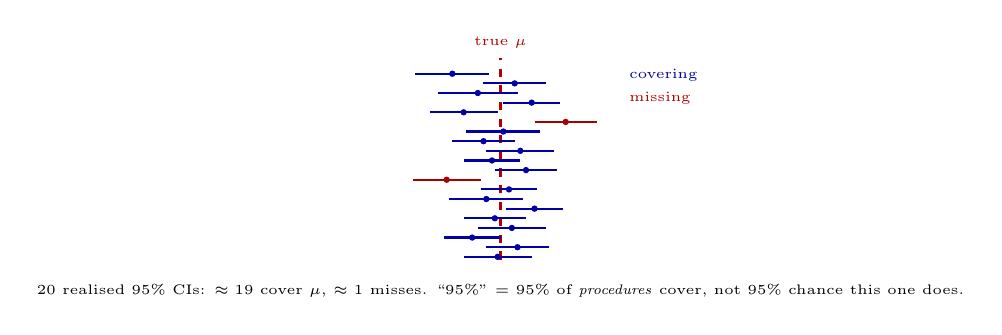
\begin{tikzpicture}[scale=0.72,every node/.style={font=\scriptsize}]
% 20 CIs, most covering true mu, a couple not
\draw[dashed,thick,red!70!black] (0,-1.6)--(0,1.95) node[above,font=\tiny] {true $\mu$};
\foreach \i/\x/\w/\col in {1/-0.85/0.65/blue,2/0.25/0.55/blue,3/-0.40/0.70/blue,4/0.55/0.50/blue,5/-0.65/0.60/blue,6/1.15/0.55/red,7/0.05/0.65/blue,8/-0.30/0.55/blue,9/0.35/0.60/blue,10/-0.15/0.50/blue,11/0.45/0.55/blue,12/-0.95/0.60/red,13/0.15/0.50/blue,14/-0.25/0.65/blue,15/0.60/0.50/blue,16/-0.10/0.55/blue,17/0.20/0.60/blue,18/-0.50/0.50/blue,19/0.30/0.55/blue,20/-0.05/0.60/blue} {
  \pgfmathsetmacro{\y}{1.85 - \i*0.17}
  \draw[thick,\col!65!black] (\x-\w,\y)--(\x+\w,\y);
  \fill[\col!65!black] (\x,\y) circle (1.6pt);
}
\node[font=\tiny,align=center] at (0,-2.15) {$20$ realised $95\%$ CIs: $\approx19$ cover $\mu$, $\approx1$ misses. ``$95\%$'' = $95\%$ of \emph{procedures} cover, not $95\%$ chance this one does.};
\node[font=\tiny,anchor=west] at (2.1,1.65) {\color{blue!65!black} covering};
\node[font=\tiny,anchor=west] at (2.1,1.25) {\color{red!70!black} missing};
\end{tikzpicture}
\caption{Twenty $95\%$ confidence intervals from independent samples. About $5\%$ miss the true mean---exactly what $95\%$ coverage means.}
\label{fig:ci-coverage}
\end{figure}

\subsection{Small $n$, Normal Data: $t$-Interval}
If $X_i\sim\mathcal{N}(\mu,\sigma^2)$ with $\sigma$ unknown and $n$ small,
\[
\bar X\pm t_{n-1,\,1-\alpha/2}\cdot\frac{S}{\sqrt{n}},
\]
with $t_{n-1}$ (Student's $t$, heavier tails than Normal). As $n\to\infty$, $t_{n-1}\to z$.

\subsection{CI for a Proportion}
$\hat p=S/n$, $\mathrm{Var}(\hat p)=p(1-p)/n$. Wald interval: $\hat p\pm z_{1-\alpha/2}\sqrt{\hat p(1-\hat p)/n}$ (needs $n\hat p(1-\hat p)\ge5$). Better: Wilson or Clopper--Pearson for small $n$.

\subsection{Sample-Size Planning}
To get margin $m=z\cdot\sigma/\sqrt{n}\le m_0$, need $n\ge(z\sigma/m_0)^2$.
For proportions, worst-case $p=1/2$ gives $n\ge(z/(2m_0))^2$;
for $m_0=0.03$ at $95\%$, $n\ge1068$.
For $m_0=0.01$ at $95\%$, $n\ge9604$---quadrupling precision quadruples $n$ (CLT $1/\sqrt{n}$ rate).

% ============================================================
\section{Bootstrap and Modern Intervals (Outlook)}
\label{sec:bootstrap}
When CLT conditions are doubtful (skewed data, small $n$, complex statistics), the \emph{bootstrap} resamples the data with replacement to simulate the sampling distribution directly. Procedure: draw $B$ bootstrap samples $X_1^*,\dots,X_n^*$ from the empirical distribution, compute $\hat\theta^*_b$ each time, then take quantiles of $\{\hat\theta^*_b\}$. No formula for $\mathrm{Var}(\hat\theta)$ needed---the resamples estimate it. Bootstrap CIs (percentile, BCa) are standard in ML evaluation (e.g., confidence bands for accuracy). Cross-validation and permutation tests follow the same ``simulate the null/sampling world'' idea and connect to hypothesis testing (Ch.~8).

\begin{remark}[When to bootstrap vs.\ $t$] Bootstrap wins for medians, trimmed means, or $R^2$ where closed-form SE is messy; $t$/$z$ win when Normality holds and $n$ is moderate, giving shorter, exact intervals without resampling cost. Rule of thumb: if $n\ge30$ and data roughly symmetric, $t$ is fine; otherwise bootstrap.
\end{remark}

% ============================================================
\section{Computing Estimators in Code}
\label{sec:code-estimation}

\begin{lstlisting}[language=Python]
import random, math

# Simulate CIs for Normal mean: coverage check
def ci_normal_mean(data, alpha=0.05):
    n = len(data)
    mean = sum(data)/n
    s = math.sqrt(sum((x-mean)**2 for x in data)/(n-1))
    z = 1.96  # for 95%, large n; use t_{n-1} for small n
    half = z*s/math.sqrt(n)
    return mean-half, mean+half

true_mu, true_sigma, n = 10.0, 2.0, 30
hits = 0
for _ in range(10000):
    data = [random.gauss(true_mu, true_sigma) for _ in range(n)]
    lo, hi = ci_normal_mean(data)
    if lo <= true_mu <= hi: hits += 1
print(f"Empirical coverage: {hits/10000:.3f} (target 0.950)")

# MLE for Bernoulli: sample proportion
data_bern = [1,1,0,1,0,0,1,1,1,0]
p_hat = sum(data_bern)/len(data_bern)
print(f"Bernoulli MLE p_hat = {p_hat:.2f}")

# Bootstrap CI for the mean (percentile method)
def bootstrap_ci(data, B=5000, alpha=0.05):
    n = len(data)
    means = [sum(random.choices(data, k=n))/n for _ in range(B)]
    means.sort()
    lo = means[int((alpha/2)*B)]
    hi = means[int((1-alpha/2)*B)]
    return lo, hi
print("Bootstrap 95% CI:", bootstrap_ci([random.gauss(10,2) for _ in range(30)]))
\end{lstlisting}

% ============================================================
\section{Chapter Notes}
Fisher (1922, 1925) created MLE and the modern CI framework (with Neyman, 1937). Student (Gosset, 1908) derived the $t$-distribution for small-sample brewing data. The ``$95\%$ chance the true value is in this interval'' misreading is the most common statistical error in computing papers---always say ``$95\%$ of such intervals cover.''

% ============================================================
\section{Exercises}
\label{sec:ch07-exercises}
\begin{enumerate}[label=E7.\arabic*, leftmargin=*, itemsep=0.8em]
\item \textbf{Bias and MSE.} $X_i\sim\mathcal{N}(\mu,\sigma^2)$. Compare estimators $\hat\mu_1=\bar X$ and $\hat\mu_2=\frac1{n+1}\sum X_i$ (shrunk). Compute bias, variance, MSE of each. For what $\mu$ does $\hat\mu_2$ win on MSE?
\item \textbf{MLE for Poisson.} Derive the MLE $\hat\lambda$ for i.i.d.\ $\mathrm{Pois}(\lambda)$ via log-likelihood. Is it unbiased? What is its variance? Simulate $n=20$, $\lambda=3$ to verify.
\item \textbf{CI construction.} $n=25$ Normal samples give $\bar x=42.3$, $s=5.1$. Construct $95\%$ $t$-CI for $\mu$ (use $t_{24,0.975}=2.064$). How does it compare to the $z$-interval? Why is $t$ wider?
\item \textbf{Proportion CI.} In $n=200$ trials, $58$ successes. Give $95\%$ Wald CI for $p$. Check the $n\hat p(1-\hat p)$ condition. What $n$ is needed for margin $\pm0.02$ at $95\%$ (worst case)?
\item \textbf{Interpretation trap.} A $95\%$ CI for latency is $[41,47]\,$ms. A colleague says ``$P(41\le\mu\le47)=0.95$.'' Explain why this is wrong, what is random vs.\ fixed, and how to phrase it correctly.
\end{enumerate}
% End of Chapter 7
